\documentclass{panikzettel}

\usepackage{hanging}
\usepackage{xifthen}

\title{Lineare Algebra Panikzettel}
\author{Mathis Müller, Philipp Schröer, Tobias Polock,\\ Jonathan du Mesnil de Rochemont, Caspar Zecha}

% Formatting
\relpenalty=9999
\binoppenalty=9999

% Definitions
\newlength{\hangwidth}
\newcommand{\skript}[1]{\settowidth{\hangwidth}{\textbf{(#1)} }\hangpara{\hangwidth}{1}\textbf{(#1)} \ignorespaces} % Für Referenzen auf das Skript. Benutzung: \skript{Stelle} Inhalt

\newcommand{\End}{\mathrm{End}} % Menge der Endomorphismen
\newcommand{\id}{\mathrm{id}} % Die Identitätsfunktion
\newcommand{\Sol}{\mathrm{Sol}} % Lösungsraum
\newcommand{\Col}{\mathrm{Col}} % Spaltenraum
\newcommand{\rk}{\mathrm{rk}} % Rang
\newcommand{\defekt}{\mathrm{def}} % Defekt
\newcommand{\GL}{\mathrm{GL}} % Lineare Gruppe
\newcommand{\Map}{\mathrm{Map}} % Menge der Funktionen
\newcommand{\Pol}{\mathrm{Pol}} % Menge der Polynomfunktionen
\newcommand{\Ker}{\mathrm{Ker}} % Kern
\renewcommand{\Im}{\mathrm{Im}} % Bild
\newcommand{\Field}{\mathbb{F}} % Endlicher Körper
\newcommand{\Eig}{\mathrm{Eig}} % Eigenraum
\newcommand{\geo}{\mathrm{g}} % Geometrische Vielfachheit
\newcommand{\mul}{\mathrm{m}} % Algebraische Vielfachheit
\newcommand{\pr}{\mathrm{pr}} % Projektion
\newcommand{\scp}[2]{\langle\ifthenelse{\isempty{#1}}{-}{#1},\ifthenelse{\isempty{#2}}{\ifthenelse{\isempty{#1}}{=}{-}}{#2}\rangle} %  Skalarprodukt. Beide Argumente können leer gelassen werden, um partielle Anwendung (wie im Skript) auszudrücken.
\newcommand{\conj}[1]{\overline{#1}} % Complexe Konjugation
\newcommand{\Interpol}{\mathrm{Interpol}} % Menge der Interpolationen
\newcommand{\Prox}{\mathrm{Prox}} % Menge der besten Approximationen
\newcommand{\ApprSol}{\mathrm{ApprSol}} % Menge der besten Näherungslösungen
\newcommand{\Fit}{\mathrm{Fit}} % Menge der Ausgleichsfunktionen
\newcommand{\SolRec}{\mathrm{SolRec}} % Menge der Lösungen zu einer HALRG oder einem HALRGsystem.
\newcommand{\C}{\mathbb{C}}
\newcommand{\R}{\mathbb{R}}
\newcommand{\N}{\mathbb{N}}
\newcommand{\inv}[1]{#1^{-1}}
\newcommand{\transpose}[1]{#1^{\mathrm{tr}}}
\newcommand{\adjoint}[1]{#1^{\mathrm{ad}}}
\newcommand{\ortho}{\bot}
\newcommand{\Intpol}{\mathrm{Intpol}}

\begin{document}

\maketitle

\setcounter{tocdepth}{2}
\tableofcontents

\section{Einleitung}

Dieser ``Panikzettel'' für Lineare Algebra ist eine mehr oder weniger informelle Zusammenfassung des Skriptes der Vorlesung Lineare Algebra im SS 2017 von \href{http://www.math.rwth-aachen.de/~Sebastian.Thomas/photo.jpg}{Dr. Sebastian Thomas}. Es werden hier die wichtigsten Aussagen, Tipps und Erklärungen gesammelt, die hoffentlich in dem unvermeidbaren Moment der Panik bei Hausaufgaben oder beim Lernen helfen. Wir haben etwas Formalismus im Sinne der Übersichtlichkeit weggelassen, wie etwa offensichtliche $n \in \mathbb{N}$.

Dieser Panikzettel kommt ursprünglich aus dem SS 2016 und wird im Laufe der Vorlesung aktualisiert. Referenzen beziehen sich auf das neue Skript vom 23. April 2017.

Dieses Projekt ist lizenziert unter \href{https://creativecommons.org/licenses/by-sa/4.0/}{CC-BY-SA-4.0} und wird auf dem Git-Server der RWTH verwaltet: \url{https://git.rwth-aachen.de/philipp.schroer/panikzettel}

\newpage
\section{Vektorräume und ihre Homomorphismen}

$K$-Vektorraum $V$ hat die Operationen Addition  $V \times V \to V, (v,w) \mapsto v+w$, sowie die Skalarmultiplikation $K \times V \to V, (a,v) \mapsto a \cdot v  $, für den folgende Axiome mit $v, w, x \in V, a,b \in K$ gelten müssen:

\begin{enumerate}
\item Assoziativität d. Addition: $(v+w)+x = v+(w+x)$
\item Nullvektor: $\exists 0 \in V: v+0=0+v=v$
\item Negative: $(-v)+v=v+(-v)=0$
\item Kommutative Additon: $v+w=w+v$
\item Assoziative Skalarmultiplikation: $a(bv)=(ab)v$
\item Einselement: $1\cdot v=v$
\item Distributivität: $(a+b)v=(av)+(bv)$, sowie $a(v+w)=(av)+(aw)$
\end{enumerate}

\subsection{Untervektorräume}

\skript{1.10} Für $K$-Vektorräume $U$ und $V$ heißt $U$ Untervektorraum von $V$, wenn die Menge der Vektoren von $U$ Teilmenge der Menge der Vektoren von $V$ ist und für $k \in K, u,u^\prime \in U$ gilt:
\begin{align*}
	u {+}^{U} u^\prime &= u {+}^{V} u^\prime	\\
	k \cdot^{U} u^\prime &= k \cdot^{V} u^\prime
\end{align*}

Wir schreiben $U \leq V$ für ``$U$ ist ein Untervektorraum von $V$'' und $U \nleq V$ für ``$U$ ist kein Untervektorraum von $V$''.

\skript{1.13} Man kann zeigen, dass eine Teilmenge $U$ eines $K$-Vektorraums $V$ ein Untervektorraum von $V$ ist, indem man für alle $a \in K,\ u,u^\prime \in U$ zeigt:
\begin{enumerate}
	\item $u+u^\prime \in U$
	\item $0 \in U$
	\item $au \in U$
\end{enumerate}
oder
\begin{enumerate}
	\item $U \neq \emptyset$
	\item $au+u^\prime \in U$.
\end{enumerate}

\subsection{Linearkombinationen und Lineare Unabhängigkeit}

Eine Linearkombination eines Tupels $s = (s_1,s_2, \ldots, s_n)$ in einem $K$-Vektorraum $V$ ist eine Summe der Einträge von $s$ mit Vorfaktoren aus $K$.

Ein Tupel heißt linear unabhängig, wenn kein Eintrag eine Linearkombination der anderen Einträge ist.

\subsection{Erzeugendensysteme, Basen und Dimension}

Ein Tupel $s$ in Vektorraum $V$ ist Erzeugendensystem von $V$, wenn jedes Element von $V$ eine Linearkombination von $s$ ist.

Für ein Tupel $s$ in $V$ ist das Erzeugnis $\langle s \rangle$ die Menge aller Linearkombinationen von $s$. Das Erzeugnis eines beliebigen Tupels in einem $K$-Vektorraum $V$ ist ein Untervektorraum von $V$.

Ein linear unabhängiges Erzeugendensystem wird Basis genannt. Gibt es eine endliche Basis von $V$ der Länge $n$, dann nennen wir $V$ endlich erzeugt und sagen, dass $V$ Dimension $n$ hat.

\skript{1.48} (Basisergänzungssatz) Jedes linear unabhängige Tupel in einem endlich erzeugten Vektorraum kann zu einer Basis dieses Vektorraums ergänzt werden.

\subsection{Unabhängigkeit von Untervektorräumen und innere direkte Summe}

\skript{1.67} Für einen $K$-Vektorraum $V$ und Untervektorräume $U_1,\ldots,U_n$ von $V$ ist die innere Summe von $(U_1,\ldots,U_n)$:
$$ U_1 + \ldots + U_n =  \sum_{i = 1}^n U_i := \left\{ \sum_{i=1}^n u_i \vert u_i \in U_i \right\}$$
Sind für jedes $u \in U_1 + \ldots + U_n$ die $u_i \in U_i$ mit $u = \sum_{i=1}^n u_i$ eindeutig gegeben, heißt $(U_1,\ldots,U_n)$ unabhängig. In diesem Fall nennen wir die innere Summe auch innere direkte Summe, geschrieben
$$ U_1 \dot+ \ldots \dot+ U_n = \dot\sum_{i=1}^n U_i := \sum_{i=1}^n U_i$$

\skript{1.70} Für $n$-Tupel $s = (s_1,\ldots,s_n)$ in $V$ gilt:
\begin{enumerate}
	\item $\langle s_1,\ldots,s_n\rangle = \sum_{i=1}^{n} Ks_i$
	\item $s$ ist Erzeugendensystem von V genau dann wenn $V = \sum_{i=1}^n Ks_i$ ist.
	\item $s$ ist linear unabhängig genau dann wenn alle $s_i \neq 0$ sind und $(Ks_1,\ldots,Ks_n)$ unabhängig ist.
	\item $s$ ist eine Basis von V genau dann wenn alle $s_i \neq 0$ sind und $V = \dot\sum_{i=1}^n K s_i$  gilt.
\end{enumerate}

\skript{1.72} Ein Tupel $(U_1,\ldots,U_n)$ von Untervektorräumen von $V$ ist unabhängig genau dann wenn für alle $i \in \mathbb{N}, i \le n$ gilt: $U_i \cap \sum_{j \in \{1,\ldots,n\}\setminus\{i\}} U_j = \{0\}$

Insbesondere sind zwei Untervektorräume $U_1$ und $U_2$ unabhängig genau dann wenn $U_1 \cap U_2 = \{0\}$ ist.

\skript{1.76} Für einen $K$-Vektorraum $V$ und Untervektorräume $(U_1,\ldots,U_n)$ mit $V = \dot\sum_{i=1}^n U_i$ bzgl. $(U_1,\ldots,U_n)$ ist die Projektion von $V$ auf $U_i$ definiert als
$$ \pr_i: V \to U_i, \left(\sum_{i=1}^n u_i\right) \mapsto u_i \text{ für } u_i \in U_i$$

\skript{1.78} Für einen Untervektorraum $U$ von $V$ heißt $U^\prime$ Komplement von $U$ wenn $V = U \dot+ U^\prime$ gilt.

\subsection{Homomorphismen}

\skript{2.2} Ein Vektorraumhomomorphismus ist eine Funktion $\varphi : V \to W$ zwischen zwei Vektorräumen, welche die folgenden äquivalenten Bedingungen erfüllt:
\begin{itemize}
\item Für $a \in K, v, v^\prime \in V$:
	\begin{enumerate}
		\item Additivität: Für $v, v^\prime \in V$ ist $\varphi(v + v^\prime) = \varphi(v) + \varphi(v^\prime)$
		\item Homogenität: Für $a \in K, v \in V$ ist $\varphi(av) = a \varphi(v)$
	\end{enumerate}
\item Für $a \in K, v, v^\prime \in V$ ist $\varphi(av + v^\prime) = a \varphi(v) + \varphi(v^\prime)$
\end{itemize}

\skript{2.5} Ein Vektorraum\textbf{\underline{endo}}morphismus von $V$ ist ein Vektorraum\textbf{\underline{homo}}morphismus von $V$ nach $V$.

\skript{2.9} Ein Vektorraum\textbf{\underline{iso}}morphismus ist ein bijektiver/invertierbarer Vektorraum\textbf{\underline{homo}}morphismus.

\skript{2.10} Ein Vektorraum\textbf{\underline{auto}}morphismus ist ein Vektorraum\textbf{\underline{iso}}morphismus von $V$ nach $V$. \\Andere Namen: $\textrm{GL}(V) = \textrm{Aut}(V) = \textrm{Aut}_K(V) := \textrm{End}_K(V)^\times$

\subsubsection{Bild und Kern, Rang und Defekt}

Es seien $K$-Vektorräume $V$ und $W$ und ein $K$-Vektorraumhomomorphismus $\varphi: V \to W$.

\skript{2.11a} $\Im \varphi$ ist ein $K$-Untervektorraum von $W$.

\skript{2.11b} $\Ker \varphi \coloneqq \{v \in V | \varphi(v)=0 \}$ ist ein $K$-Untervektorraum von $V$.

\skript{2.21a} $\defekt_K(\varphi) \coloneqq \dim_K(\Ker\varphi)$

\skript{2.21b} $\rk_K(\varphi) \coloneqq \dim_K(\Im\varphi)$

\subsubsection{Rangsatz}

\skript{2.27} Für jeden $K$-Vektorraumhomomorphismus $\varphi: V \to W$ gilt: $$\dim_K(V) = \rk_K(\varphi) + \defekt_K(\varphi)$$

\subsubsection{Verschiedenes}

Es seien $K$-Vektorräume $V$ und $W$, ein $K$-Vektorraumhomomorphismus $\varphi: V \to W$ und ein Tupel $s \in K^n$.

\skript{2016 Aufg. 24c} $\varphi(\langle s_1,\ldots,s_n \rangle) = \langle \varphi(s_1), \ldots, \varphi(s_n) \rangle$

\skript{2016 Aufg. 24de} Wenn $(\varphi(s_1),\ldots,\varphi(s_n))$ linear unabhängig ist, dann ist auch $(s_1,\ldots,s_n)$ linear unabhängig. Ist $\varphi$ injektiv, so gilt auch die Umkehrung.

% Anwendung: Interpolation

\section{Matrixkalkül}

\subsection{Spalteninterpretation}

% Größe von B?
Für $m,n \in \mathbb{N}_0, A \in K^{m \times n}$:

\skript{3.1} $\varphi_A: K^{n \times 1} \to K^{m \times 1}, x \mapsto Ax$

\skript{3.4} $\varphi_A(x) = \sum_{j =1}^n  x_j A_{-,j}$

\skript{3.5 a} $\varphi_{BA}=\varphi_B \circ \varphi_A$

\skript{3.5 b} $\varphi_{\mathrm{E}_n} = \id_{K^{n \times 1}}$

\skript{3.5 c} $\varphi_{A}^{-1}=\varphi_{A^{-1}}$

\subsection{Koordinatenspalte}

\skript{3.6} Für eine Basis $s$ von $V$ ist $\kappa_s : V \to K^{n \times 1}$\\ der zu $K^{n \times 1} \to V, a \mapsto \sum_{i \in [1,n]} a_i s_i$ inverse VR.-Iso.

Für $\kappa_s(v)$ muss also das LGS $\sum_{i \in [1,n]} a_i s_i = v$ gelöst werden, dann sind $a_i = \kappa_s(v)_i$.

\subsection{Darstellungsmatrix}

\skript{3.8} Für VR-Hom. $\varphi : V \to W$, Basis $s = (s_1, \ldots, s_n)$ von $V$ und Basis $t = (t_1, \ldots, t_m)$ von $W$ ist $M_{t,s}(\varphi)$ die Darstellungsmatrix zu $s$ und $t$:
$$\mathrm{M}_{t,s}(\varphi) = (\kappa_t(\varphi(s_1)) \ldots \kappa_t(\varphi(s_n)))$$

Es muss also für jede Spalte $i$ das $s_i$ in $\varphi$ eingesetzt werden und das Ergebnis wieder nach den Linearfaktoren von $t$ aufgelöst werden.

\skript{Tutoraufgabe 30.5.16 a} $\mathrm{M}_{e,e}(\varphi_A) = A$

\subsection{Basiswechselmatrix, Basiswechselformeln}

\skript{3.15} Die Darstellungsmatrix $\mathrm{M}_{s, s^\prime}(\id_V)$ wird Basiswechselmatrix von $s$ nach $s^\prime$ genannt.

Achtung: $\mathrm{M}_{s, s^\prime}(\id_V) \cdot v$ übersetzt ein $v$ von $s^\prime$ zu $s$! Die Bezeichnung ``von $s$ nach $s^\prime$'' ist also rückwärts. Dies wird mit praktischer Verwendung begründet.

\skript{3.18a} Mit Basen $s = (s_1,\ldots, s_n)$ und $s^\prime = (s^\prime_1, \ldots, s^\prime_n)$ von $V$ gilt für $v \in V$:\\ $\kappa_{s^\prime}(v) = (\mathrm{M}_{s,s^\prime}(\id_V))^{-1} \kappa_s(v)$.

\skript{3.18b} Mit VR-Hom. $\varphi : V \to W$, Basen $s = (s_1,\ldots, s_n)$ und $s^\prime = (s^\prime_1, \ldots, s^\prime_n)$ von $V$ und Basen $t = (t_1,\ldots, t_n)$ und $t^\prime = (t^\prime_1, \ldots, t^\prime_n)$ von $W$ gilt: \\
$\mathrm{M}_{t^\prime, s^\prime}(\varphi) = (\mathrm{M}_{t,t^\prime}(\id_W))^{-1} \mathrm{M}_{t,s}(\varphi) \mathrm{M}_{s,s^\prime}(\id_V)$

\subsection{Kardinalitäten von verschiedenen Mengen}

$$\abs{\Sol(A,0)} = q^{n-r} \text{ für } A \in \Field_q^{m \times n} \text{ mit } \rk_{\Field_q} A = r$$
Da Elemente aus $\Sol(A,0)$ Vektoren aus $\Field_q^n$ sind, müssen wir $n$ Parameter aus $\Field_q$ wählen, von denen $r$ nicht frei sind.

$$\abs{\{ U \leq \Field_q^n | \dim_{\Field_q} U = k \}} = \binom{n}{k}_q$$
$\binom{n}{k}_q$ ist der Gauß'sche Binomialkoeffizient.

$$\abs{\mathrm{Hom}(\Field_q^n,\Field_q^m)} = \abs{\Field_q^{m \times n}} = q^{m \cdot n}$$
Homomorphismen lassen sich als Matrizen darstellen und umgekehrt. Daher machen wir auch das ganze Matrixkalkül-Zeugs.

$$\abs{\GL_n(\Field_q)} = \prod_{i=0}^{n-1} q^n-q^i$$
$$\abs{\{A \in \Field_q^{m \times n} ~ | ~ \rk(A) = \min(m,n)\}} = \prod_{i=0}^{\min(m,n)-1} (q^{\max(m,n)}-q^i)$$
Wir müssen Zeilen oder Spalten linear unabhängig wählen, genau $\min(m,n)$ Stück mit Länge $\max(m,n)$. Die erste Zeile/Spalte ist dann bis auf den Nullvektor frei zu wählen, danach sollte jede folgende kein Vielfaches der vorherigen sein.

\subsection{Anwendung: Interpolation}
\skript{3.A} Für eine Menge $X$, einen Körper $K$ und ein $a \in X^m$ schreiben wir
$$\varepsilon_a:\Map(X,K) \to K^m, f \mapsto (f(a_1),\dots,f(a_m)).$$

\skript{3.C + 3.D} Für eine Menge $X$, einen Körper $K$, eine Teilmenge $S$ von $\Map(X,K)$ und zwei Tupel $a \in X^m$, $b\in K^m$ ist die \textit{Menge der Interpolationen} zu $(a,b)$ in $S$ gegeben durch
$$\Intpol_S(a,b):=(\varepsilon_a|_S)^{-1}(\{b\}) = \set{f \in S \;|\; f(a_i) = b_i \text{ für } i \in [1,m]}.$$
Informell: Interpolationen sind die Abbildungen $f$ aus $S$, für die stets $f(a_i)=b_i$ für $i \in [1,m]$ gilt.

\skript{3.K} Für eine Menge $X$, einen $K$-Untervektorraum $U$ von $\Map(X,K)$, eine Basis $s$ von $U$ und zwei Tupel $a \in X^m,\ b \in K^m$ ist
$$\Intpol_U(a,b)=\{\sum_{j=1}^{n}c_j s_j \;|\; c \in \Sol(
	\left(\begin{array}{ccc}
	s_1(a_1)& \dots & s_n(a_1)	\\
	\vdots & &  \vdots	\\
	s_1(a_m) & \dots & s_n(a_m)
	\end{array}\right),
	\left(\begin{array}{cc}
	b_1 &\\
	\vdots &\\
	b_m &\\
	\end{array}\right)
	)\}.$$
Damit lässt sich die Menge der Interpolationen durch das Lösen eines LGS bestimmen. Ist\\ $U = \Pol_{<n}(K,K)$, bietet sich die Basis $s=(s_1,\dots,s_n)$ mit $s_j : K \rightarrow K, x \mapsto x^{j-1}$ an. Links im LGS steht dann die Vandermonde-Matrix $V(a)$.

\subsection{Ähnlichkeit und Äquivalenz}

\skript{3.43} \begin{itemize}
	\item Für $A, B \in K^{m \times n}$ ist $A$ äquivalent zu $B$, wenn es $P \in \GL_n(K)$, $Q \in \GL_m(K)$ gibt mit: $$Q^{-1} A P = B$$
	\item Für $A, B \in K^{n \times n}$ ist $A$ ähnlich zu $B$, wenn es $P \in \GL_n(K)$ gibt mit: $$P^{-1} A P = B \iff A P = P B$$
\end{itemize}

\skript{3.50} Für $\varphi : V \to W$ sollen Basen $(s_1, \ldots, s_n)$ von $V$ und $(t_1, \ldots, t_m)$ von $W$ bestimmt werden, sodass $M_{t,s}(\varphi) = Q_r$ eine Quasieinheitsmatrix ist mit $r \leq \min(n, m)$. Dann rechnen wie folgt: \begin{enumerate}
    \item Basis $(t_1, \ldots, t_r)$ von $\Im \varphi$ berechnen.
    \item Zur Basis von $V$ erweitern: $(t_1, \ldots, t_n)$.
    \item Urbilder $s_j$ von Bildbasis berechnen: $t_j = \varphi(s_j)$ für $j \in [1, r]$.
    \item Basis $(s_{r+1}, \ldots, s_n)$ von $\Ker \varphi$ bestimmen.
\end{enumerate}

\skript{3.52} Für $A, B \in K^{m \times n}$ ist $A$ genau dann äquivalent zu $B$, wenn $$\rk(A) = \rk(B)$$

Mit unserem Wissen von Eigenwerten können wir Ähnlichkeit durch folgenden Entscheidungsbaum prüfen. Der Baum sieht groß und kompliziert aus, ist aber eine schnelle Methode insbesondere um Ähnlichkeit zu widerlegen. Falls alle Bedingungen eines Knotens erfüllt sind, gehe weiter zum linken Kind, sonst zum rechten Kind.

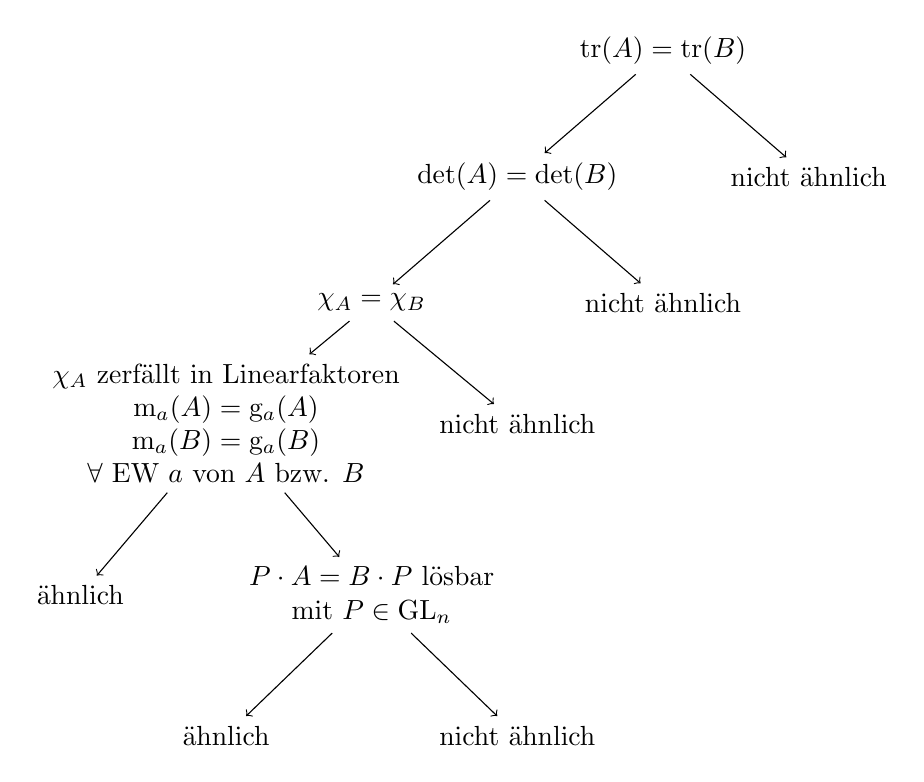
\begin{tikzpicture}[
		->, level distance=1.3cm, sibling distance=3.7cm, growth parent anchor=south
	]
	\node {$\textrm{tr}(A) = \textrm{tr}(B)$}
		child { node {$\det(A) = \det(B)$}
			child { node {$\chi_A = \chi_B$}
				child { node[align=center] {$\chi_A$ zerfällt in Linearfaktoren \\ $\mul_a(A) = \geo_a(A)$ \\ $\mul_a(B) = \geo_a(B)$ \\ $\forall$ EW $a$ von $A$ bzw. $B$}
					child { node {ähnlich} }
					child { node[align=center] {$P \cdot A = B \cdot P$ lösbar \\ mit $P \in \GL_n$}
						child { node { ähnlich } }
						child { node {nicht ähnlich} }
					}
				}
				child { node {nicht ähnlich}}
			}
			child { node {nicht ähnlich}}
		}
		child { node {nicht ähnlich} };
\end{tikzpicture}

Für Bonusaufgaben, ist es teilweise notwendig die Ähnlichkeit nicht diagonalisierbarer Matrizen zu zeigen. Wahrscheinlich sind die angegebenen Matrizen dann trigonalisierbar und insb. ähnlich zu ihrer Jordan-Normalform. Die \href{https://de.wikipedia.org/wiki/Jordansche_Normalform}{\textbf{Wikipedia-Seite zur Jordan-Normalform}} ist hier sehr hilfreich. Zuletzt sei noch auf ein \href{http://www.math.rwth-aachen.de/~Sebastian.Thomas/teaching/lineare_algebra_ii_09/Beispiel_Jordan-Normalform.pdf}{\textbf{Beispiel von Sebastian Thomas aus LA2 zur Jordan-Normalform}} hingewiesen.

\section{Lineare Kodierungstheorie}

\subsection{Blockcode}

\skript{4.1} Blockcode: Nicht-leere Teilmenge $C$ von $K^{n \times 1}$ über $K$ mit Länge $n$. Elemente von $C$ werden Codewörter genannt.

\skript{4.3} Hamming-Gewicht: $\mathrm{wt}(a):=|\{i \in [1,n]|a_i \neq 0\}|$ mit $a \in K^{n \times 1}$

\skript{4.5c} $\mathrm{wt}(a+b) \leq \mathrm{wt}(a)+ \mathrm{wt}(b)$

\skript{4.6} Hamming-Abstand: $d(a,b):=wt(b-a)$

\skript{4.7} \begin{itemize} \item $\mathrm{d}(a,b)=|\{i \in [1,n]|a_i \neq b_i\}|$
	\item $\mathrm{d}(a,c) \leq \mathrm{d}(a,b)+\mathrm{d}(b,c)$
\end{itemize}

\skript{4.10} Offene Kugel: $\mathrm{B}_r(a):=\{x \in K^{n \times 1}|\mathrm{d}(a,x) < r\}$ mit $r \in \mathbb{R}_{\geq 0}$.\\Abgeschlossene Kugel analog mit $\leq$.

\subsection{Minimalabstand eines Blockcodes}

\skript{4.12} Minimalabstand: $\mathrm{d}(C):=\min\{\mathrm{d}(c,c^\prime)|c,c^\prime \in C$ mit $c \neq c^\prime \}$, falls $|C| \ge 1$
\begin{itemize}
	\item $\mathrm{B}_{\mathrm{d}(C)}(c) \cap C = \{c\}$
\end{itemize}

\skript{4.15} Nächster Nachbar von $x$ ist $c$ mit $\mathrm{d}(c,x)=\min\{d(c^\prime,x|c^\prime \in C)\}$
\begin{itemize}
	\item $\forall x \in \mathrm{B}_{\frac{\mathrm{d}(C)}{2}}(c)$ ist $c$ der eindeutige nächste Nachbar von $x \in C$
\end{itemize}

\subsection{Lineare Codes}

\skript{4.19} $C \leq K^{n \times 1}$ ist ein linearer $[n,k,d]$-Code, wenn die Länge $n$, $\dim_K C=k$ und $\mathrm{d}(C)=d$ ist.

\skript{4.21} $\mathrm{d}(C) = \min \{\mathrm{wt}(c)|c \in C\setminus\{0\}\}$, falls $C \neq \{0\}$ sonst $0$.

\subsection{Erzeugermatrizen}

\skript{4.22} Eine Erzeugermatrix ist $A \in K^{n \times k}$ mit $C=\Col(A)$, wenn C ein linearer $[n,k]$-Code über $K$ ist.

\skript{4.24} $\rk_K A=k$, falls $A$ Erzeugermatrix für linearen  $[n,k]$-Code $C$.

\skript{4.25} Kodierung und Dekodierung:
\begin{itemize}
	\item Kodieren von $w \in K^{k \times 1}$ zu einem Codewort mit Erzeugermatrix $A$: \\
	Berechne $Aw$.
	\item Dekodieren eines Codewortes $c \in C$ zu einem Informationswort bzgl. $A$.: \\
	Berechne $w \in K^{k \times 1}$ mit $Aw=c$.
\end{itemize}

\subsection{Kontrollmatrizen}

\skript{4.26} Kontrollmatrix ist $B \in K^{(n-k) \times n}$ mit $C=\Sol(B,0)$, wenn $k \in [0,n], C$ ein linearer $[n,k]$-Code über $K$ ist.
\begin{itemize}
	\item Berechnung der Kontrollmatrix $C$ mit Erzeugermatrix $A: \Sol(A^{tr},0)=\langle u,..,v\rangle=\Col(B^{tr})$.
	\item $\Sol(B,0)=\Col(A)=C$.
\end{itemize}

\skript{4.28} $rk_K B=n-k$.

\skript{4.29} Codewort-Test: Berechne $Bx$ und falls $Bx=0$ ist, dann ist $x$ ein Codewort von $C$.

\skript{4.30} Seien $k \in [1,n],$ ein linearer $[n,k]$-Code $C$ über $K$ und die Kontrollmatrix $B$ gegeben. Dann ist \\
$\mathrm{d}(C) = \min \{r \in \mathbb{N}_0 \ |\ $ es gibt $j_1,...,j_r \in [1,n]$ mit $j_1 <...<j_r$ so, dass $(B_{-,j_1},...,B_{-,j_r})$ linear abhängig ist\}\\
=$ \max \{r \in \mathbb{N}_0 \ |\ $ für alle $j_1,...,j_{r-1} \in [1,n]$ mit $j_1 <...<j_{r-1}$ ist $(B_{-,j_1},...,B_{-,j_{r-1}})$ linear unabhängig\}.

\subsection{Syndromdekodierung}

\skript{4.31} Syndrom: Für $x \in K^{n \times 1}$ heißt $Bx \in K^{(n-k) \times 1}$ das Syndrom von $x$ bzgl. $B$, mit $k \in [1,n]$ und einem linearen $[n,k]$-Code $C$ über $K$.

\skript{4.33} Sei $y$ das Syndrom von $x$. Für $x^\prime \in K^{n \times 1}$ gilt: $x^\prime$ hat das Syndrom $y \Leftrightarrow x^\prime-x$ ist ein Codewort von $C$.

\skript{4.34} Ein Anführer für $y$ bzgl. $B$ ist ein $e \in K^{n \times 1}$ mit Syndrom $y$ und $\mathrm{wt}(e)=\min\{\mathrm{wt}(x)\ |\ x \in K^{n \times 1}$ so, dass $x$ das Syndrom $y$ hat$\}$.

\skript{4.36} Codewort $c$ ist ein nächster Nachbar von $x$ mit Syndrom $y$ in $C \Leftrightarrow x-c$ ist Anführer für $y$.

\skript{4.37} $\forall x \in B_{\frac{d(C)}{2}}(c)$ ist $x-c$ der eindeutige Anführer für das Syndrom von $x$.

\skript{4.38} Syndromdekodierung: \\

Initialisierung:
\begin{itemize}
	\item Wähle $k \in [0,n]$ und einen linearen $[n,k]$-Code $C$ über $K$, mit weniger als $\frac{d(C)}{2}$ Fehlern.
	\item Bestimme die Kontrollmatrix $B$ für $C$
	\item Bestimme $\forall y \in K^{(n-k) \times 1}$ einen Anführer $e_y$ und lege ein Wörterbuch an
\end{itemize}
Dekodierung von $x \in K^{n \times 1}$:
\begin{itemize}
	\item Berechne das Syndrom $Bx$ von $x$ bzgl. $B$
	\item Suche Fehlerwort $e_{Bx}$ aus Wörterbuch
	\item Dekodiere $x$ zu $x-e_{Bx}$
\end{itemize}

Beachte: Gibt es für ein Syndrom $y$ mehrere Anführer, so lassen sich $x \in K^{n \times 1}$ mit Syndrom $y$ nicht eindeutig dekodieren.

\section{Determinante}

Die Determinante gibt Auskunft über quadratische Matrizen. Visuell entspricht die Determinante von $A$ der (gerichteten) Änderung von Volumen durch $\phi_A$. Wenn sie invertierbar ist, dann ist auch die Matrix invertierbar. In Körpern heißt das einfach ungleich Null, in Ringen muss Invertierbarkeit genauer geprüft werden. Im Folgenden ist $R$ ein beliebiger kommutativer und unitärer Ring.

Die Leibniz-Formel für kleine Matrizen:

\skript{5.2a} Für $A \in R^{0 \times 0}$: $\det \begin{pmatrix} & \end{pmatrix} = 1$

\skript{5.2b} Für $A \in R^{1 \times 1}$: $\det A = A_{1,1}$

\skript{5.3c} Für $A \in R^{2 \times 2}$: $\det A = A_{1,1} A_{2,2} - A_{1,2} A_{2,1}$ \\

\skript{5.15} \textit{Kästchensatz.} Für Matrizen $A \in R^{m \times m}$, $B \in R^{m \times n}$, $C \in R^{n \times n}$ gilt: \\
$\det \begin{pmatrix} A & B \\ 0 & C \end{pmatrix} = (\det A) (\det C)$

Der Kästchensatz ist der beste Ansatz, um Determinanten größerer Matrizen per Hand auszurechen: Man vereinfacht die Matrix (siehe Abschnitt zur Veränderung der Matrix) und dann wendet man den Kästchensatz an.

\subsection{Produktsatz}

\skript{5.8a} $\det (B A) = (\det B) (\det A)$

\skript{5.8b} $\det \textrm{E}_n = 1$

\skript{5.8c} $(\det A)^{-1} = \det (A^{-1})$

\subsection{Matrixoperationen und die Determinante}

\skript{5.4} $\det \transpose{A} = \det A$

\skript{5.5/1} \textit{Multilinearität.} \begin{itemize}
\item $\begin{aligned}
	& \det \begin{pmatrix} x_1 & \ldots & x_{k-1} & y+z & x_{k+1} & \ldots  & x_n \end{pmatrix} = \\
		& \hspace{2em} \det \begin{pmatrix} x_1 & \ldots & x_{k-1} & y & x_{k+1} & \ldots  & x_n \end{pmatrix} +
		\det \begin{pmatrix} x_1 & \ldots & x_{k-1} & z & x_{k+1} & \ldots  & x_n \end{pmatrix}
 \end{aligned}$
\item $\det \begin{pmatrix} x_1 & \ldots & x_{k-1} & ay & x_{k+1} & \ldots  & x_n \end{pmatrix} = a \det \begin{pmatrix} x_1 & \ldots & x_{k-1} & y & x_{k+1} & \ldots  & x_n \end{pmatrix}$
\end{itemize}

\skript{5.5/2} Wenn zwei Spalten gleich sind, dann gilt $\det A = 0$.

Um die Determinante deutlich einfacher berechnen zu können, ist es möglich, die Matrix mit unseren elementaren Zeilen- und Spaltenoperationen (via 5.4) zu vereinfachen.

\skript{5.6a} Mit $k \neq l$: $\det \textrm{sw}_{k,l}(A) = - \det A$

\skript{5.6b} Mit $a \in R$ und $k \neq l$: $\det \textrm{add}_{k,l,a}(A) = \det A$

\skript{5.6c} Mit $a \in R$: $\det \textrm{mul}_{k,a}(A) = a \det A$

\subsection{Laplace-Entwicklung}

Determinanten größerer Matrizen werden in der Praxis mit der Laplace-Entwicklung rekursiv berechnet. Bei Berechnung der Determinante per Hand sollte man wenn möglich aber die obigen Sätze benutzen, da die Laplace-Entwicklung fehleranfällig ist.

Für die Laplace-Entwicklung brauchen wir die Definition des Minor:

\skript{5.11} Mit $(k,l)$ und $k,l \in [1,n]$ und $A \in R^{n \times n}$:\\ $\textrm{Minor}_{k,l}(A) = \det A^\prime$ wobei $A^\prime$ einfach $A$ ohne Zeile $k$ und Spalte $l$ ist.

Die Laplace-Entwicklung kann man dann entweder nach einer Spalte $l$ oder nach einer Zeile $k$ durchführen:

\begin{minipage}{0.45\textwidth}
\skript{5.13a} Für Spalte $l \in [1,n]$: \\
$$\det A = \sum_{k=1}^n (-1)^{k+l} A_{k,l} \textrm{Minor}_{k,l}(A)$$
\end{minipage}\hspace{0.05\textwidth}
\begin{minipage}{0.45\textwidth}
\skript{5.13b} Für Zeile $k \in [1,n]$: \\
$$\det A = \sum_{l=1}^n (-1)^{k+l} A_{k,l} \textrm{Minor}_{k,l}(A)$$
\end{minipage}

Die Laplace-Entwicklung in Worten:

\begin{enumerate}
\setcounter{enumi}{-1}
\item \textit{Pro-Tipp:} Vorher die Matrix mit elementaren Zeilenoperationen vereinfachen. Vergleiche Korollar (5.6).
\item Zeile oder Spalte aussuchen, nach der man entwickeln möchte. Am Besten wählt man hier eine Zeile/Spalte mit vielen Nullen, das spart gleich Arbeit.
\item Jedes Element der gewählten Zeile/Spalte wird dann mit einem Minor multipliziert. Der Minor ist einfach die Determinante, wo Zeile und Spalte des aktuellen Elementes weggestrichen wurden. Hier profitiert man von den Nullen.
\item Gegebenenfalls für den Minor rekursiv weiter Laplace-Entwickeln.
\item Für jedes Element der gewählten Zeile/Spalte nun Wert und Minor multiplizieren und alternierend addieren. Genau dann wenn die entwickelte Zeile/Spalte geraden Index hat, beginnt man mit $(-1)$.
\end{enumerate}

\subsection{Determinante eines Vektorraumendomorphismus}

Man beachte: Vektorraum\textbf{\underline{endo}}morphismus.

Die Determinante ist unabhängig von den Basen der Darstellungsmatrix:

\skript{5.9} Für  $\varphi : V \to V$, Basen $s = (s_1, \ldots, s_n), s^\prime = (s^\prime_1, \ldots, s^\prime_n)$ von $V$ gilt: \\
$\det \textrm{M}_{s,s}(\varphi) = \det \textrm{M}_{s^\prime, s^\prime}(\varphi)$ \\

Damit können wir auch problemlos $\det \textrm{M}_{s,s}(\varphi)$ mit $\det \varphi$ abkürzen.

\section{Eigenwerte}

Ein Eigenvektor $v$ eines Endomorphismus $\varphi$ ist ein Vektor $\neq 0$, der von dem Endomorphismus bis auf einen skalaren Faktor, den Eigenwert $a$, nicht verändert wird: $\varphi(v) = a v$.

\skript{6.1} Ein Eigenraum ist der Vektorraum, der alle Eigenvektoren zu einem Eigenwert (und den Nullvektor) enthält.
$$\Eig_a(\varphi) = \{ v \in V \vert \varphi(v) = a v \} = \Ker(\varphi - a \cdot \id_V)$$
Beachte: Wir nennen $\Eig_a(\varphi)$ genau dann einen Eigenraum, wenn $\Eig_a(\varphi)\neq \{0\}$ ist.\\
Die Eigenwerte/-vektoren/-räume einer Matrix $A$ sind die Eigenwerte/-vektoren/-räume von $\varphi_A$.

\skript{6.6} Für verschiedene Eigenwerte sind die zugehörigen Eigenräume unabhängig.

\subsection{Charakteristische Polynome}

\skript{6.8} Das charakteristische Polynom einer Matrix $A$ ist $\chi_A = \det(XE_n-A)$.

\skript{6.12} Das charakteristische Polynom eines Vektorraumendomorphismus $\varphi$ ist $\chi_\varphi = \chi_{M_{s,s}(\varphi)}$ für eine beliebige Basis $s$.

\skript{6.13} Es sind äquivalent: \begin{itemize}
	\item $a$ ist ein Eigenwert von $A$
	\item $\rk(A-aE_n)<n$
	\item $\det(A-aE_n)=0$
	\item $a$ ist eine Nullstelle des charakteristischen Polynoms von $A$.
\end{itemize}

\subsubsection{Begleitmatrix}

\skript{6.20} Für ein normiertes Polynom $f = X^n + \sum_{i=0}^{n-1} a_iX^i \in K[X]\setminus\{0\}$ ist die Begleitmatrix
$$C(f) = \left(\begin{array}{cccc}
		& 0 & & -a_0	\\
		& & & -a_1	\\
		& E_{n-1} & & \vdots	\\
		& & & -a_{n-1}
\end{array}\right)$$

\skript{6.22} Das charakteristische Polynom einer Begleitmatrix ist $\chi_{C(f)} = f$.

\subsection{Vielfachheiten}

\skript{6.16} Die geometrische Vielfachheit eines Eigenwertes $a$ von einem Endomorphismus $\varphi$ ist
$$\geo_a(\varphi) = \dim(\Eig_a(\varphi))$$
	Die algebraische Vielfachheit eines Eigenwertes $a$ von einem Endomorphismus $\varphi$ ist
$$\mul_a(\varphi) = \mul_a(\chi_\varphi)$$
	Für eine Matrix $A$ sind Vielfachheiten analog über $\varphi_A$ gegeben.

\skript{6.19} Es gilt stets $\geo_a(\varphi) \le \mul_a(\varphi)$.


\subsection{Anwendung: PageRank}

\subsubsection{Stochastische Matrizen}

\skript{6.27} Es ist $A \in \mathbb{R}^{m \times n}$ stochastisch, wenn alle Einträge in $A$ nicht-negativ sind und für $j \in [1,n]$ stets $\sum_{i\in [1,m]} A_{i,j}=1 $ gilt.

\skript{6.29} Für stochastische $A,B \in \mathbb{R}^{m \times n}$ und $c \in [0,1]_\mathbb{R}$ ist auch $$cA+(1-c)B$$ stochastisch.

\skript{6.30} Quadratische stochastische Matrizen besitzen stets den Eigenwert 1.

\skript{6.31} Quadratische stochastische Matrizen mit positiven Einträgen besitzen genau einen stochastischen Eigenvektor zum Eigenwert 1, dieser hat nur positive Einträge.

\subsubsection{PageRank}

Für eine Ecke $j$ in einem schlichten gerichteten Graphen $G$ ist $$\Gamma_+(j) = \{i \in \text{V}(G)\ |\ \text{es gibt eine Kante von } j \text{ nach } i\}$$ und $\deg_+(j)=|\Gamma_+(j)|$.

\skript{6.32} Für einen schlichten gerichteten Graphen $G$ mit $\text{V}(G)=[1,n]$ heißt $L \in \mathbb{R}^{n \times n}$ die Linkmatrix gegeben durch
$$L_{i,j}=\begin{cases}
\frac{1}{\deg_+(j)}, & \text{falls } i \in \Gamma_+(j) \\
0, & \text{sonst}
\end{cases}$$

\skript{6.36} Für einen schlichten gerichteten Graphen $G$ mit $\text{V}(G)=[1,n]$ mit Linkmatrix $L$, $S \in \mathbb{R}^{n \times n}$ gegeben durch
$$S=\left(\begin{array}{ccc}
1& \dots & 1	\\
\vdots & &  \vdots	\\
1 & \dots & 1
\end{array}\right)$$
und $D \in \mathbb{R}^{n \times n}$ gegeben durch
$$D_{i,j}=\begin{cases}
0, & \text{falls } \deg_+(j) > 0 \\
1, & \text{sonst}
\end{cases}$$
und $d \in [0,1]_\mathbb{R}$ ist $P_d$ die Googlematrix von G zum Dämpfungsfaktor $d$ gegeben durch
$$P_d = d (L + \frac{1}{n} D) + (1-d) \frac{1}{n} S.$$

\skript{6.39} Für einen schlichten gerichteten Graphen $G$ mit $\text{V}(G)=[1,n]$ und $d \in [0,1)_\mathbb{R}$ und der zugehörigen Googlematrix $P_d$ ist der PageRank der eindeutige stochastische Eigenvektor von $P_d$ zum Eigenwert 1.

\subsection{Diagonalisierbarkeit}

Die folgenden Definitionen gelten für Endomorphismen $\varphi$, sowie für quadratische Matrizen mithilfe der Spalteninterpretation $\varphi_A$.

\skript{6.41} Eine Basis $s$ von $V$ ist eine Eigenbasis bezüglich $\varphi$, wenn alle Einträge von $s$ Eigenvektoren von $\varphi$ sind.

\skript{6.43} Für einen Endomorphismus $\varphi: V \to V$ ist eine Basis $s$ von $V$ genau dann eine Eigenbasis bezüglich $\varphi$, wenn $M_{s,s}(\varphi)$ eine Diagonalmatrix ist.

\skript{6.45} Für eine Basis $s$ der Länge $n$ ist jedes $s_i$ genau dann ein Eigenvektor zum Eigenwert $a_i$ von Matrix $A \in K^{n \times n}$, wenn mit $P = ( s_1 \ldots s_n )$ gilt:
\[
	P^{-1} A P = \begin{pmatrix}
	    a_{1} &        & 0    \\
	          & \ddots &      \\
	    0     &        & a_{n}
	  \end{pmatrix}
\]

\skript{6.46} $\varphi$ ist diagonalisierbar, falls es eine Eigenbasis bezüglich $\varphi$ gibt.

\skript{6.50} Für eine Matrix $A \in K^{n \times n}$ sind äquivalent: \begin{itemize}
	\item $A$ ist diagonalisierbar.
	\item Es gibt eine Eigenbasis bezüglich $A$.
	\item $A$ ist ähnlich zu einer Diagonalmatrix.
\end{itemize}

\skript{6.52} Für einen Endomorphismus $\varphi: V \to V$ sind äquivalent: \begin{itemize}
	\item $\varphi$ ist diagonalisierbar.
	\item $V = \dot\sum_{a \in K\text{, a ist Eigenwert von } \varphi}\ \Eig_a(\varphi)$.
	\item $\dim V = \sum_{a \in K} \geo_a(\varphi)$.
	\item Das charakteristische Polynom $\chi_\varphi$ zerfällt in Linearfaktoren und für jeden Eigenwert $a$ von $\varphi$ gilt $\geo_a(\varphi) = \mul_a(\varphi)$.
\end{itemize}

\skript{6.53} Wenn ein Endomorphismus $\varphi: V \to V$ genau $\dim V$ verschiedene Eigenwerte hat, ist er diagonalisierbar.

\skript{6.56} Für $f \in K[X]$, $A \in K^{n \times n}$ und $P \in \GL_n(K)$ gilt:	\\
Wenn
\[A = P \left(\begin{array}{ccc}
		a_1 & & 0	\\
		& \ddots &	\\
		0 & & a_n
	\end{array}\right) P^{-1}\]
ist, dann ist
$$f(A) = P \left(\begin{array}{ccc}
		f(a_1) & & 0	\\
		& \ddots &	\\
		0 & & f(a_n)
	\end{array}\right) P^{-1}$$
	
\subsection{Anwendung: Homogene autonome lineare Rekursionsgleichungen}

Eine \textit{homogene autonome lineare Rekursionsgleichung} (HALRG) von Grad $n$ über $K$ in den Unbekannten $x_k$ mit $i \in [0, n-1]$, ist durch $$x_{k+n} = \sum_{i \in [0,n-1]} a_ix_{k+1}$$ für $k \in \N_0$ gegeben.

Das charakteristische Polynom einer HALRG von Grad $n$ über $K$ ist $$X^n - \sum_{i \in [0, n-1]}a_i X^i$$.

\skript{6.70} Sei ein normiertes $f \in K[X]\backslash\{0\}$ mit $\deg{f} = n$ gegeben. Dann ist der Lösungsraum zur HALRG mit charakteristischem Polynom $f$ gegeben durch $$\SolRec(f) = \set{ (((\transpose{C(f)})^k c)_1)_{k\in\N_0} \;|\; c \in K^{n \times 1} }.$$

\skript{6.71} Sei $f \in K[X], a_0, a_1 \in K$ mit $f = X^2 - a_1X - a_0 = (X - b_1)(X - b_2)$ und $b_1 \neq b_2$ gegeben.  Für $x \in K^{\N_0}$ gilt dann $$x_{k+2} = a_0x_k + a_1x_{k+1} \iff x_k = \frac{b_1^kb_2 - b_2^kb_1}{b_2 - b_1}x_0 + \frac{b_2^k - b_1^k}{b_2 - b_1}x_1$$ für $k \in \N_0$.

Offenbar ist 6.71 nur für HALRGen mit charakteristischem Polynom $f$ von Grad 2 anwendbar, für die $f$ in Linearfaktoren zerfällt.

\subsection{Invariante Untervektorräume}

\skript{6.77} Für einen Vektorraumendomorphismus $\varphi: V \to V$ ist ein Untervektorraum $U$ von $V$ invariant unter $\varphi$, wenn
$\varphi(U) \subseteq U$.

\skript{6.78} Für einen $K$-Vektorraumendomorphismus $\varphi: V \to V$ und einen Untervektorraum $U$ von $V$ mit einer Basis $s = (s_1,\ldots, s_n)$, sodass $s^\prime = (s_1,\ldots,s_m)$ ($m \leq n$) eine Basis von $U$ ist, ist $U$ invariant unter $\varphi$ genau dann, wenn die Darstellungsmatrix von $\varphi$ zu $s$ die Form
$$M_{s,s}(\varphi) = \left(\begin{array}{cc}
		A & B	\\
		0 & C
	\end{array}\right)$$
mit $A \in K^{m \times m}$ hat. In diesem Fall ist $M_{s^\prime,s^\prime}(\varphi\vert_U^U) = A$.

\skript{6.80} Für einen $K$-Vektorraumendomorphismus $\varphi: V \to V$ und einen $\varphi$-invarianten Untervektorraum $U$ von $V$ gilt $\chi_{\varphi\vert_U^U} \vert \chi_\varphi$, d.h. das charakteristische Polynom von $\varphi$ eingeschränkt auf $U$ teilt das charakteristische Polynom von $\varphi$.

\subsubsection{Satz von Cayley/Hamilton}
\skript{6.81} \begin{enumerate} \item Für einen $K$-Vektorraumendomorphismus $\varphi: V \to V$ gilt: $\chi_\varphi(\varphi) = 0$.
	\item Für eine Matrix $A \in K^{n \times n}$ gilt: $\chi_A(A) = 0$.
\end{enumerate}

\section{Skalarprodukträume}

Skalarprodukträume betrachten wir nur über den Körpern $\C$ und $\R$. Daher ist im folgenden stets $K \in \{\C,\R\}$.

\subsubsection{Adjungierte}
\skript{7.A} Für eine Matrix $A \in K^{m \times n}$ ist die dazugehörige \textit{adjungierte Matrix} $\adjoint{A} \in K^{m \times n}$ definiert als:
$$ \adjoint{A} = \transpose{\conj{A}} = \conj{\transpose{A}} = (\conj{A_{i,j}})_{j \in \left[ 1,n \right], i \in \left[ 1,m \right]} $$
Falls $K = \R$, so entspricht diese Operation dem Transponieren. Es gelten die gleichen Regeln wie für das Transponieren bis auf die Skalarmultiplikation. Für diese gilt: $\adjoint{cA} = \conj{c}\adjoint{A}$.

\subsection{Skalarprodukt}
\skript{7.1} Ein Skalarproduktraum ist ein $K$-Vektorraum $V$ mit einer Abbildung $$\scp{}{}: V \times V \to K, (v,w) \mapsto \scp{v}{w}$$ die die folgenden Axiome erfüllt:
\begin{itemize}
	\item Sesquilinearität: Für $a \in K$, $v,w,w^\prime \in V$ ist $\scp{v}{aw+w^\prime} = a \scp{v}{w} + \scp{v}{w^\prime}$ und $\scp{aw+w^\prime}{v} = \conj{a}\scp{w}{v} + \scp{w^\prime}{v}$.
	\item Hermitizität: Für $v,w \in V$ gilt: $\scp{v}{w} = \conj{\scp{w}{v}}$.	\\
		Im Fall von $K = \R$ gilt also $\scp{v}{w} = \scp{w}{v}$.	\\
		Im Fall von $K = \C$ folgt, dass das Skalarprodukt eines Vektors mit sich selbst reell ist: $\scp{v}{v} = \conj{\scp{v}{v}}$.
	\item Positive Definitheit: Für $v \in V$ gilt $\scp{v}{v} \geq 0$ und genau dann $\scp{v}{v} = 0$ wenn $v = 0$ ist.
\end{itemize}

\skript{7.4} Solange nichts anderes erwähnt ist, betrachten wir $K^n$ mit dem Standardskalarprodukt gegeben durch
$$ \scp{v}{w} = \transpose{\conj{v}} w = \sum_{i=1}^n \conj{v_i} w_i$$

\subsubsection{Cauchy-Schwarz-Ungleichung}
\skript{7.7} In einem $K$-Skalarproduktraum gilt für $v,w \in V$:
$$\abs{\scp{v}{w}}^2 \leq \scp{v}{v} \scp{w}{w}$$
und genau dann
$$\abs{\scp{v}{w}}^2 = \scp{v}{v} \scp{w}{w}$$
wenn $(v,w)$ linear abhängig in $V$ ist.

\subsection{Normierte Vektorräume}

\skript{7.8} Ein normierter Vektorraum ist ein $K$-Vektorraum mit einer Abbildung $\norm{-}: V \to \R, v \mapsto \norm{v}$ mit den folgenden Eigenschaften:\\
\begin{itemize}
	\item Positive Definitheit: Für alle $v \in V$ ist $$\norm{v} \ge 0$$ und genau dann $\norm{v} = 0$ wenn $v = 0$ ist.
	\item Absolut-Homogenität: Für alle $k \in K, v \in V$ ist $$ \norm{kv} = \abs{k} \norm{v}$$
	\item Dreiecksungleichung: Für alle $v,w \in V$ ist $$\norm{v+w} \le \norm{v} + \norm{w}$$
\end{itemize}

\skript{7.10} Jeder $K$-Skalarproduktraum wird zu einem normierten $K$-Vektorraum mit der Norm gegeben durch $$\norm{v} = \sqrt{\scp{v}{v}}$$

Wenn keine andere Norm angegeben ist, wird diese Norm angenommen.

\skript{7.13} Ein Vektor $v$ in einem normierten $K$-Vektorraum heißt normiert, wenn $$\norm{v} = 1$$ ist.

\skript{7.16} Für $v,w \in V$ ist $$\norm{v+w}^2 + \norm{v - w}^2 = 2\norm{v}^2 + 2\norm{w}^2$$

\skript{7.17 a)} In einem $\R$-Skalarproduktraum $V$ gilt $$\scp{v}{w} = \frac{1}{2}(\norm{v + w}^2 - \norm{v}^2 - \norm{w}^2) = \frac{1}{4}(\norm{v + w}^2 - \norm{v - w}^2)$$

\skript{7.17 b)} In einem $\C$-Skalarproduktraum $V$ gilt $$\scp{v}{w} = \frac{1}{4}(\norm{v + w}^2 - \norm{v - w}^2) + i\frac{1}{4}(-\norm{v + iw}^2 + \norm{v -iw}^2)$$

\subsection{Winkel}

\skript{7.18} In einem $\R$-Skalarproduktraum ist der Winkel zwischen zwei Vektoren $v,w \in V \setminus \{0\}$ gegeben durch $$\angle(v,w) := \arccos\left(\frac{\scp{v}{w}}{\norm{v}\norm{w}}\right)$$

\subsection{Orthogonalität}

\skript{7.20} Für $v,w \in V$ ist $v$ orthogonal zu $w$, geschrieben $v \ortho w$ wenn gilt $$\scp{v}{w} = 0.$$

\skript{7.22} Satz des Pythagoras: Für $v,w \in V$ mit $v \ortho w$ ist $$\norm{v + w}^2 = \norm{v}^2 + \norm{w}^2.$$

\skript{7.24} Für eine Teilmenge $S$ von $V$ ist $$S^\ortho := \{v \in V \vert \forall s \in S: s \ortho v\}$$ ein $K$-Untervektorraum von $V$. Dieser Vektorraum heißt Orthogonalraum zu $S$ in $V$.

\skript{7.26} In einem $K$-Skalalarproduktraum $V$ gilt für jedes $n$-Tupel $(s_1,\ldots,s_n)$ in $V$
$$\langle s_1,\ldots,s_n\rangle^\ortho = \{s_1,\ldots,s_n\}^\ortho.$$

\skript{7.27} In einem  $K$-Skalarproduktraum $V$ sind für jeden Untervektorraum $U$ von $V$ die beiden Vektorräume $(U,U^\ortho)$ unabhängig.

\skript{7.28} Für einen $K$-Untervektorraum $U$ von $V$ mit $V = U \dotplus U^\ortho$ (für endlichdimensionale $V$ ist dies stets der Fall) bezeichnet $\pr_U: V \to U$ die Projektion auf $U$ bezüglich $(U,U^\ortho)$.

\subsubsection{Orthogonalbasen}

\skript{7.30} Ein Tupel $(s_1,\ldots,s_n)$ in $V$ heißt orthogonal, wenn für alle $i,j \in \left[ 1,n\right]$ mit $i \neq j$ $s_i \ortho s_j$ gilt. Ein soches Tupel heißt orthonormal wenn es orthogonal ist und jeder eintrag normiert ist.

\skript{7.33} Ein orthogonales Tupel, das nicht die Null enthält, ist stets linear unabhängig.

\skript{7.32} Für ein Tupel $s = (s_1, \ldots, s_n)$ in $V$ mit allen $s_i \neq 0$ und einen Vektor $v \in \langle s \rangle$ mit $a \in K^n$ sodass $\sum_{i=1}^n a_i s_i = v$ gilt $$a_i = \frac{\scp{s_i}{v}}{\scp{s_i}{s_i}}$$ für alle $i \in \left[ 1,n\right]$.

\skript{7.34} Eine orthogonale Basis von $V$ heißt Orthogonalbasis von $V$. Eine orthonormale Basis von $V$ heißt Orthonormalbasis von $V$.

\skript{7.37} Parsevalscher Entwicklungssatz: Es sei $(s_1,\ldots,s_n)$ eine Orthogonalbasis von $V$. Dann gilt für $v \in V$:
$$v = \sum_{i=1}^n \frac{\scp{s_i}{v}}{\scp{s_i}{s_i}} s_i$$

\skript{7.38} Es sei ein $K$-Untervektorraum $U$ von $V$ mit einer Orthogonalbasis $(s_1,\ldots,s_n)$ von $U$ gegeben. Dann ist $V = U \dotplus U^\ortho$ und für $v \in V$ gilt:
\begin{align*}
	\pr_U(v) &= \sum_{i=1}^n \frac{\scp{s_i}{v}}{\scp{s_i}{s_i}} s_i	\\
	\pr_{U^\ortho}(v) &= v - \sum_{i=1}^n \frac{\scp{s_i}{v}}{\scp{s_i}{s_i}} s_i
\end{align*}

\subsubsection{Gram-Schmidt-Orthogonalisierung}

\skript{7.39} Es sei ein linear unabhängiges $n$-Tupel $(s_1,\ldots,s_n)$ gegeben. Dann ist ein Tupel $(t_1,\ldots,t_n)$ gegeben durch $$t_i = \pr_{\langle s_1, \ldots, s_{i-1} \rangle^\ortho}(s_i)$$ und für jedes $j \in \left[ 1,n\right]$ ist $(t_1,\ldots,t_j)$ eine Orthogonalbasis von $\langle s_1,\ldots,s_j \rangle$.

\skript{7.40} In jedem Skalarproduktraum gibt es eine Orthonormalbasis.


\subsubsection{QR-Zerlegung}

\skript{7.47} Es sei $A \in K^{m \times n}$ mit $\rk(A) = n$ gegeben. Dann sind $n$-Tupel $(t_1, \ldots, t_n)$ und $(t^\prime_1, \ldots, t^\prime_n)$ gegeben durch
\begin{align*}
	t^\prime_i &= \pr_{\langle A_{-,1},\ldots,A_{-,i-1} \rangle^\ortho}(A_{-,i})	\\
	t_i &= \frac{1}{\norm{t^\prime_i}} t^\prime_i
\end{align*}
Außerdem sind $Q \in K^{m \times n}, R \in K^{n \times n}$ gegeben durch
$$Q = (t_1 ~ \ldots ~ t_n), R = \left(\begin{array}{ccc}
\scp{t_1}{A_{-,1}}	&	\cdots	&	\scp{t_1}{A_{-,n}}	\\
	&	\ddots	&	\vdots	\\
0	&	&	\scp{t_n}{A_{-,n}}
\end{array}\right)$$
Dann heißt das Paar $(Q,R)$ die QR-Zerlegung von $A$ und es gilt $R \in \GL_n(K)$ sowie $A = QR$.


\subsection{Nichtausartung von Skalarprodukten}

\skript{7.J (a)} Für $v, v^\prime \in V$ gilt: Wenn für $w \in V$ stets $\langle v, w\rangle = \langle v^\prime, w \rangle$ gilt, dann ist $v = v^\prime.$

\skript{7.J (b)} Für $w, w^\prime \in V$ gilt: Wenn für $v \in V$ stets $\langle v, w\rangle = \langle v, w^\prime \rangle$ gilt, dann ist $w = w^\prime.$

\subsection{Adjunktion von Vektorraumhomomorphismen}

\skript{7.K} Eine \textit{Adjungierte} zu einem $K$-Vektorraumhomomorphismus $\varphi: V \rightarrow W$, ist ein \\ $K$-Vektorraumhomomorphismus $\psi: W \rightarrow V$ sodass  für $v \in V, w \in W$ stets
	$$\langle \varphi(v), w\rangle = \langle v, \psi(w)\rangle$$ gilt.

\skript{7.M} Zu jedem Vektorraumhomomorphismus gibt es höchstens eine Adjungierte. (Analog zur Inversen.)

\skript{7.N} Für einen adjungierbaren $K$-Vektorraumhomomorphismus von $V$ nach $W$ notieren wir die Adjungierte zu $\varphi$ als $\adjoint{\varphi}: W \rightarrow V$.

\skript{7.O} Bis auf die Skalarmultiplikation gelten die gleichen Rechenregeln wie für inverse Homomorphismen. Für $a \in K$ und einem adjungierbaren $K$-Vektorraumhomomorphismus $a\varphi: V \rightarrow W$ gilt: $$\adjoint{(a\varphi)} = \conj{a}\adjoint{\varphi}.$$

\skript{7.X} Es sein ein $K$-Skalarproduktraum $V$, ein adjungierbaren $K$-Vektorraumhomomorphismus $\varphi: V \rightarrow W$ und $U \leq V$ mit $V = U\,\dot{+}\,U^\ortho$ gegeben. Dann ist $U$ $\varphi$-invariant gdw. $U^\ortho$ \mbox{$\adjoint{\varphi}$-invariant} ist.

\skript{7.Y} Die Spalteninterpretation einer Matrix $A$ ist adjungierbar mit $\adjoint{\varphi_A} = \varphi_{\adjoint{A}}$.

\subsection{Beste Approximation}

\skript{7.50} Es seien eine Teilmenge $S$ von $V$ und ein Vektor $v \in V$ gegeben. Ein $s \in S$ heißt \textit{beste Approximation} von $v$ in $S$ wenn $$\norm{v - s} = \min\{\norm{v - s^\prime} \vert s^\prime \in S\}$$ gilt.

\skript{7.AA} Sei ein normierter $K$-Vektorraum $V$, $S \subseteq V$ und $v\in V$ gegeben.  $$\text{Prox}_S(v) = \{ s \in S\;|\;\norm{v - s} = \min\{ \norm{v - s^\prime}\;|\;s^\prime \in S\}\}$$ wird \textit{Menge der besten Approximationen} von $v$ in $S$ genannt.

\skript{7.54} Für einen Untervektorraum $U$ von $V$ mit $V = U \dot{+} U^\ortho$ ist $\pr_U(v)$ die eindeutige beste Approximation von $v$ in $U$.

\subsection{Anwendung: Term-Dokument-Matrizen}
Seien im Folgenden $(D_1,...,D_n)$ ein $n$-Tupel von Strings in $\left[ 1,m \right]$ und für $j \in [1,n]$ sei $l_j$ die Länge von $D_j$.

\skript{7.55} Sei $A^\prime \in \R^{m \times n}$ gegeben durch
$$A^\prime_{i,j} = |\{k \in \left[1,l_j\right]\;|\;(D_j)_k = i\}|$$ für $i\in \left[1,m\right], j \in \left[1,m\right]$. Dann wird $A^\prime$ \textit{Term-Dokument-Matrix} von $(D_1,\ldots,D_n)$ genannt. Normiert man diese Spaltenweise, so entsteht die \textit{normierte Term-Dokument-Matrix} $A \in \R^{m \times n}$. \\
\\
$A^\prime$ stellt also eine Art Häufigkeitsmatrix dar, in der die Häufigkeiten der in den Dokumenten vorkommenden Terme spaltenweise für alle Dokumente aufgeführt wird.

\skript{DS Def. (3.34)} Sei $I \subseteq [1,m]$. Dann ist $\chi_I \in \R^{m \times 1}$ der \textit{Indikatorvektor} von $I$ mit
$$\chi_{I,i} = (\chi_I)_i =
  \begin{cases}
    1, & \text{für } i \in I,\\
    0, & \text{falls } i \in [1,m]\backslash I.
  \end{cases}$$

\skript{7.57} Eine \textit{Suchanfrage} $I$ ist eine Teilmenge von $\left[ 1,m\right]$. Für $j \in \left[ 1,n\right]$ passt das Dokument $D_j$ am Besten zur Suchanfrage $I$, wenn $A_{-,j}$ eine beste Approximation von $\chi_I$ in $\{A_{-,1},...,A_{-,n}\}$ ist.

\skript{7.58} Für $j \in \left[ 1,n\right]$ passt das Dokument $D_j$ am Besten zur Suchanfrage $I$ gdw.
	$$\sum_{i \in I} A_{i,j} = \max\{\sum_{i \in I} A_{i,j^\prime} \;|\; j^\prime \in [1,n]\}.$$

\subsection{Anwendung: Beste Näherungslösungen für lineare Gleichungssysteme}

Eine Lösung für $\Sol(A,b)$ liegt immer in $\Col(A)$. Falls $b$ nicht in $\Col(A)$ enthalten ist, so müssen wir erst $b$ in den Spaltenraum von $A$ projizieren, bevor näherungsweise eine Lösung bestimmt werden kann.\\
\\
Sei $A \in K^{m \times n}$, $b \in K^{m \times 1}$ gegeben.

\skript{7.AD} $$\ApprSol(A, b) = \varphi_A^{-1}(\Prox_{\Col(A)}(b)) $$ wird \textit{Menge der besten Näherungslösungen} zur erweiterten Koeffizientenmatrix $(A\;|\;b)$ genannt.

\skript{7.AE} Diese Methode zur Bestimmung einer Näherungslösung auch \textit{Methode der kleinsten Fehlerquadrate} genannt. Und zwar aus folgendem Grund:
\begin{align*}
	\ApprSol(A, b)
	& = \{x \in K^{n \times 1}\;|\;Ax \text{ ist eine beste Approximation von } b \text{ in } \Col(A)\} \\
	& = \{x \in K^{n \times 1}\;|\; \sum_{I \in [1,m]} |b_i - Ax_1|^2 = \min\{\sum_{i \in [1,m]} |b_i - Ax_i^\prime|^2 \;|\; x^\prime \in K^{n \times 1}\}\}.
\end{align*}

\skript{7.AF} $\ApprSol(A, b) = \Sol(A, \pr_{\Col(A)}(b)) = \Sol(\adjoint{A}A, \adjoint{A}b).$

\subsection{Anwendung: Ausgleichsfunktionen}

Dieses Kapitel ist analog zur Interpolation aufgebaut. Auch hier kann es sein, dass vorgegebene Stützpunkte $(a,b)$ möglicherweise in keiner Funktion aus unserem Suchraum $S \subseteq \Map(X,K)$ als Funktionswerte auftreten. Hier bietet es sich an jede Stützstelle aus $a$ erst in den Suchraum zu projizieren, falls dieser ein Untervektorraum von $\Map(X,K)$ ist. \\
\\
Seien im Folgenden $a \in X^m$, $b \in K^n$, $S$ eine Teilmenge von $\Map(X,K)$.

\skript{7.AJ} $$\Fit_S(a,b) = (\varepsilon_a|_S)^{-1}(\Prox_{\varepsilon_a(S)}(b))$$
definiert die \textit{Menge der Ausgleichsfunktionen} zu $(a,b)$ in $S$.

\skript{7.AM} Sei $U \leq \Map(X, K)$ und $(s_1,\ldots,s_n)$ eine Basis von $U$. Dann gilt $$\Fit_U(a,b) = \{\sum_{j \in [1,n]} c_js_j \;|\; c \in \ApprSol(
\left(\begin{array}{ccc}
s_1(a_1)	&	\cdots	&	s_n(a_1)	\\
\vdots	&		&	\vdots	\\
s_1(a_m)	&	\cdots &	s_n(a_m)
\end{array}\right),
\left(\begin{array}{c}
b_1	\\
\vdots	\\
b_m
\end{array}\right) )\}.$$

\skript{7.AO} Sei $X = K$. Dann gilt $$\Fit_{\Pol<n(K,K)}(a,b) = \{K \rightarrow K, x \mapsto \sum_{j \in [1,n]} c_jx^{j-1} \;|\; c\in \ApprSol(
\left(\begin{array}{ccc}
a_1^0	&	\cdots	&	a_1^{n-1}	\\
\vdots	&		&	\vdots	\\
a_m^0	&	\cdots &	a_m^{n-1}
\end{array}\right),
\left(\begin{array}{c}
b_1	\\
\vdots	\\
b_m
\end{array}\right))\}.$$ 

Wobei die Matrix der potenzierten Stützstellen $a_1,...,a_m$ auch Vandermonde-Matrix genannt wird. Falls $\ApprSol(V,\kappa_e(b))=\Sol(V,\kappa_e(b))$, so sind die gefundenen Ausgleichsfunktionen zugleich Interpolationen. D.h. $\Fit_U(a,b) = \Interpol_U(a,b)$.

\subsection{Unitäre Matrizen}
Sei im Folgenden $V$ stets ein $K$-Skalarproduktraum.

\skript{7.AP} Die \textit{Unitäre Gruppe} von Grad $n$ über $K$ ist definiert als $$U_n(K) := \{A \in \GL_n(K) \;|\; \inv{A} = \adjoint{A}\}.$$

\skript{AR} $U_n(K) = \set{ A \in K^{n \times n} \;|\; (A_{-,1}, \ldots, A_{-,n}) \text{ ist eine Orthonormalbasis von } K^{n \times 1} }.$ 

\skript{7.AX (a)} Ein $K$-Vektorraumendomorphismus $\varphi$ heißt \textit{unitär diagonalisierbar}, falls es eine orthonormale Eigenbasis von V bezüglich $\varphi$ gibt.

\skript{7.AX (b)} Eine $(n \times n)$-Matrix Über $K$ heißt \textit{unitär diagonalisierbar}, falls es eine orthonormale Eigenbasis von $K^{n \times 1}$ bzgl. $\varphi_A$ gibt.

\subsection{Normale Endomorphismen}
Sei in diesem Abschnitt $V$ stetes ein $K$-Skalarproduktraum.

\skript{7.BC (a)} Die Menge der \textit{normalen} $K$-\textit{Vektorraumendomorphismen} ist definiert als $$\End_{\text{norm}}(V) = \End_{K,\text{norm}}(V) := \{ \varphi \in \End_K(V) \;|\; \adjoint{\varphi} \circ \varphi = \varphi \circ \adjoint{\varphi} \}.$$

\skript{7.BC (b) + 7.BD} Die Menge der \textit{normalen} $(n \times n)$-\textit{Matrizen} ist $$K_{\text{norm}}^{n \times n} = \{A \in K^{n \times n} \;|\; \varphi_A \in End_{k,\textit{norm}}(K^{n \times 1}) \} = \{ A \in K^{n \times n} \;|\; \adjoint{A}A = A\adjoint{A}\}.$$

\skript{7.BF} $U_n(K) \subset K_\text{norm}^{n \times n}$.

\skript{7.BG} Sei $\varphi: V \rightarrow V$ ein $K$-Vektorraumendomophismus.
\begin{enumerate}
	\item $\varphi$ ist normal.
	\item Für $v,w \in V$ gilt: $\scp{\adjoint{\varphi(v)}}{\adjoint{\varphi(w)}} = \scp{\varphi(v)}{\varphi(w)} $.
	\item Für $v \in V$ gilt: $\norm{\adjoint{\varphi}(v)} = \norm{\varphi(v)}$.
\end{enumerate}

\skript{7.BM} (Spektralsatz). Es sei $V$ endlichdimensional und ein $K$-Vektorraumendomorphismus $\varphi:V \rightarrow V$ gegeben. $$\varphi \text{ ist unitär diagonalisierbar } \iff \chi_\varphi \text{ zerfällt in Linearfaktoren und } \varphi \text{ ist normal}.$$

\subsection{Hermitesche Endomorphismen}
Sei im Folgenden $V$ stets ein $K$-Skalarproduktraum.

\skript{7.BN (a)} Die Menge der \textit{hermitschen} $K$-\textit{Vektorraumendomorphismen} ist definiert als
 $$\End_{\text{herm}}(V) = \End_{K,\text{herm}}(V) := \{\varphi \in \End_K(V) \;|\; \varphi \text{ ist adjungierbar und } \adjoint{\varphi} = \varphi\}.$$
 
\skript{7.BN (b) + 7.BO} Die Menge der \textit{hermitschen} $(n \times n)$-\textit{Matrizen} über $K$ ist $$K_\text{herm}^{n \times n} = \{A \in K^{n \times n} \;|\; \varphi_A \in \End_{K,\text{herm}}(K^{n \times 1})\} = \{A \in K^{n \times n} \;|\; \adjoint{A} = A\}.$$

\skript{7.BQ} $\End_{\text{herm}}(V) \subset \End_{\text{norm}}(V).$

\skript{7.BR} Sei ein hermitescher $K$-Vektorraumendomorphismus $\varphi: V \rightarrow V$ gegeben. Dann ist jeder Eigenwert von $\varphi$ reell.

\skript{7.BT} (Spektralsatz für hermitesche Endomorphismen). Jeder hermitesche Vektorraumendomorphismus ist unitär diagonalisierbar.

\subsection{Singulärwertzerlegung}
%TODO Definition Singulärwerttupel  und Singulärwertmatrix 
\skript{7.BU} Sei ein adjungierbarer $K$-Vektorraumhomomorphismus $\varphi$ gegeben. Dann ist $\adjoint{\varphi} \circ  \varphi$ hermitesch.

\skript{7.CE} Sei $A \in K^{m \times n}$ gegeben. Dann ist $A$ unitär äquivalent zu $\Sigma_{\sigma(A)} \in K^{m \times n}$. 

\skript{7.CF} Seien $A, B \in K^{m \times n}$ gegeben. $$A \text{ ist unitär äquivalent zu } B \iff \sigma(A) = \sigma(B).$$  

\end{document}


